\chapter{Operations}\label{ch:operations}

This chapter presents the operations implemented in the VisionFlow system.
The service operations were divided into two categories, each represented by a grpc protobuf contract~\cite{grpc-protobuf}, with the following features:

\begin{itemize}
    \item \textbf{Functional Operations}: operations that are part of the main functionality of the system (e.g., uploading images, retrieving processed information);
    \item \textbf{Elasticity Management}: operations that allow the system to scale up or down the available resources (i.e., the number of instances of the gRPC server and the image processing application).
\end{itemize}


\section{Functional Operations}\label{sec:functional_operations}

\subsection{Contract}\label{subsec:functional-operations-contract}

\subsection{Design Aspects}\label{subsec:functional-operations-design-aspects}


\section{Elasticity Management}\label{sec:elasticity_management}

Elasticity management is a key aspect of cloud computing.
It allows the system to adapt to the workload by scaling up or down the resources, depending on the demand.
This is important to ensure that the system is able to handle the workload efficiently and cost-effectively.

For this project,
elasticity management was implemented as a mandatory requirement for scaling instances of both the gRPC server and the image processing application
(\textit{labelsApp}), granting the clients the ability to request the scaling of these services.

\subsection{Contract}\label{subsec:elasticity-management-contract}

The elasticity management service was implemented as a gRPC service with the contract shown in Figure~\ref{fig:grpc-scaling-contract}.

\begin{figure}[!htb]
    \centering
    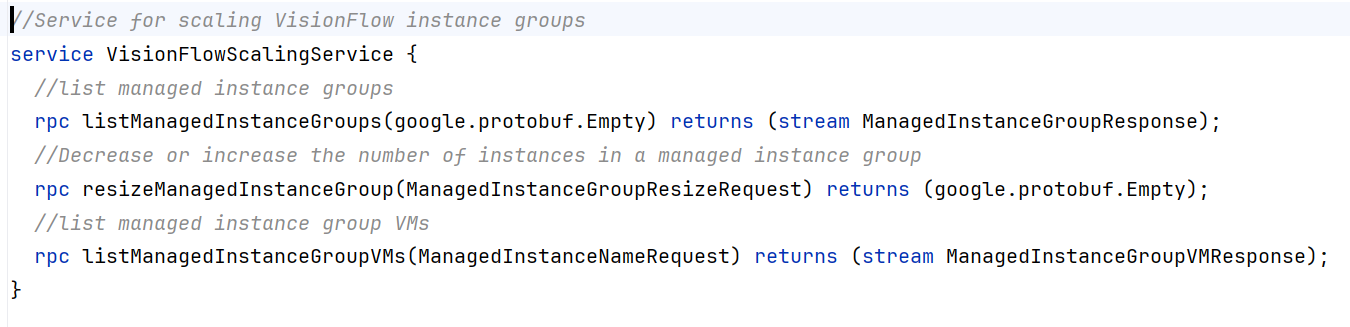
\includegraphics[width=0.8\textwidth]{../figures/grpc-scaling-contract}
    \caption{Elasticity Management Contract}
    \label{fig:grpc-scaling-contract}
\end{figure}

The contract provides the following RPC methods:

\begin{itemize}
    \item \textbf{listManagedInstanceGroups}: lists all managed instance groups.
    For this operation,
    the client does not need to provide any additional information
    and the server will return a stream of \texttt{ManagedInstanceGroupResponse} messages.
    This information can be used to identify the instance groups that can be managed for scaling and listing VMs;
    \item \textbf{resizeManagedInstanceGroup}: resizes a managed instance group.
    The client must provide the name of the managed instance group and the new size;
    \item \textbf{listManagedInstanceGroupVMs}: lists all VMs in a managed instance group.
    The client must provide the name of the managed instance group, and the server will return a stream of \texttt{ManagedInstanceGroupVMResponse} messages.
\end{itemize}

The following messages are used in the contract:

\begin{itemize}
    \item \textbf{ManagedInstanceGroupRequest} and \texttt{ManagedInstanceGroupResponse}:
    contains the \textbf{name} of a managed instance group.
    Even though both messages represent the same information, they are used in different contexts,
    and as such, they were defined as separate messages to increase the readability of the contract;
    \item \textbf{ManagedInstanceGroupResizeRequest}:
    contains the \textbf{name} of a managed instance group and the \textbf{new size} for the group;
    \item \textbf{ManagedInstanceGroupVMResponse}: contains the \textbf{name} and \textbf{status} of a VM instance.
\end{itemize}

\subsection{Design Aspects}\label{subsec:elasticity-management-design-aspects}

The grpc contract for the elasticity management service was designed
to allow for instance management and listing without depending on a specific instance group.

The client can request the list of managed instance groups and then request additional operations such as resizing or listing VMs in a specific instance group.
This way, the contract won't need to be altered if more instance or less instance groups are added to the system in the future.

However, the server implementation will need to be updated to handle the new instance groups,
as that information is stored locally.
In a real-world scenario, this information should be stored in a database or a cloud service, as the server can also be managed by the elasticity management service,
which would lead to inconsistencies across the system.
Additionally, there's no dynamic update support for the instance groups available if stored locally.

In the contract, the decision to stream the responses made by the server in the listing operations,
was made to allow the potential clients to process the information as it arrives,
instead of waiting for the entire response to be sent by the server.
